\section{Methods}

\subsection{Transformers}

In the works of NLP, the use of pre-entrained language models hace become a useful block to get a better result on every task. One of the most competitive neural sequence transduction models have an encoder-decoder structure\cite{Bahdanau_2014,Cho_2014}. Here, the encoder maps an input sequence of symbol representations $(x_1 , \dots, x_n)$ to a sequence of continuous representations $z = (z_1 , \dots, z_n )$. Given z, the decoder then generates an output sequence $(y_1 , \dots, y_m )$ of symbols one element at a time. At each step the model is auto-regressive\cite{Graves_2013}, consuming the previously generated symbols as additional input when generating the next. The Transformer follows this overall architecture using stacked self-attention and point-wise, fully connected layers for both the encoder and decoder (figure \ref{fig:transformer}). The encoder is composed of a stack of N = 6 identical layers. Each layer has two sub-layers. The first is a multi-head self-attention mechanism, and the second is a simple, position wise fully connected feed-forward network.

\begin{figure}[H]
    \centering
    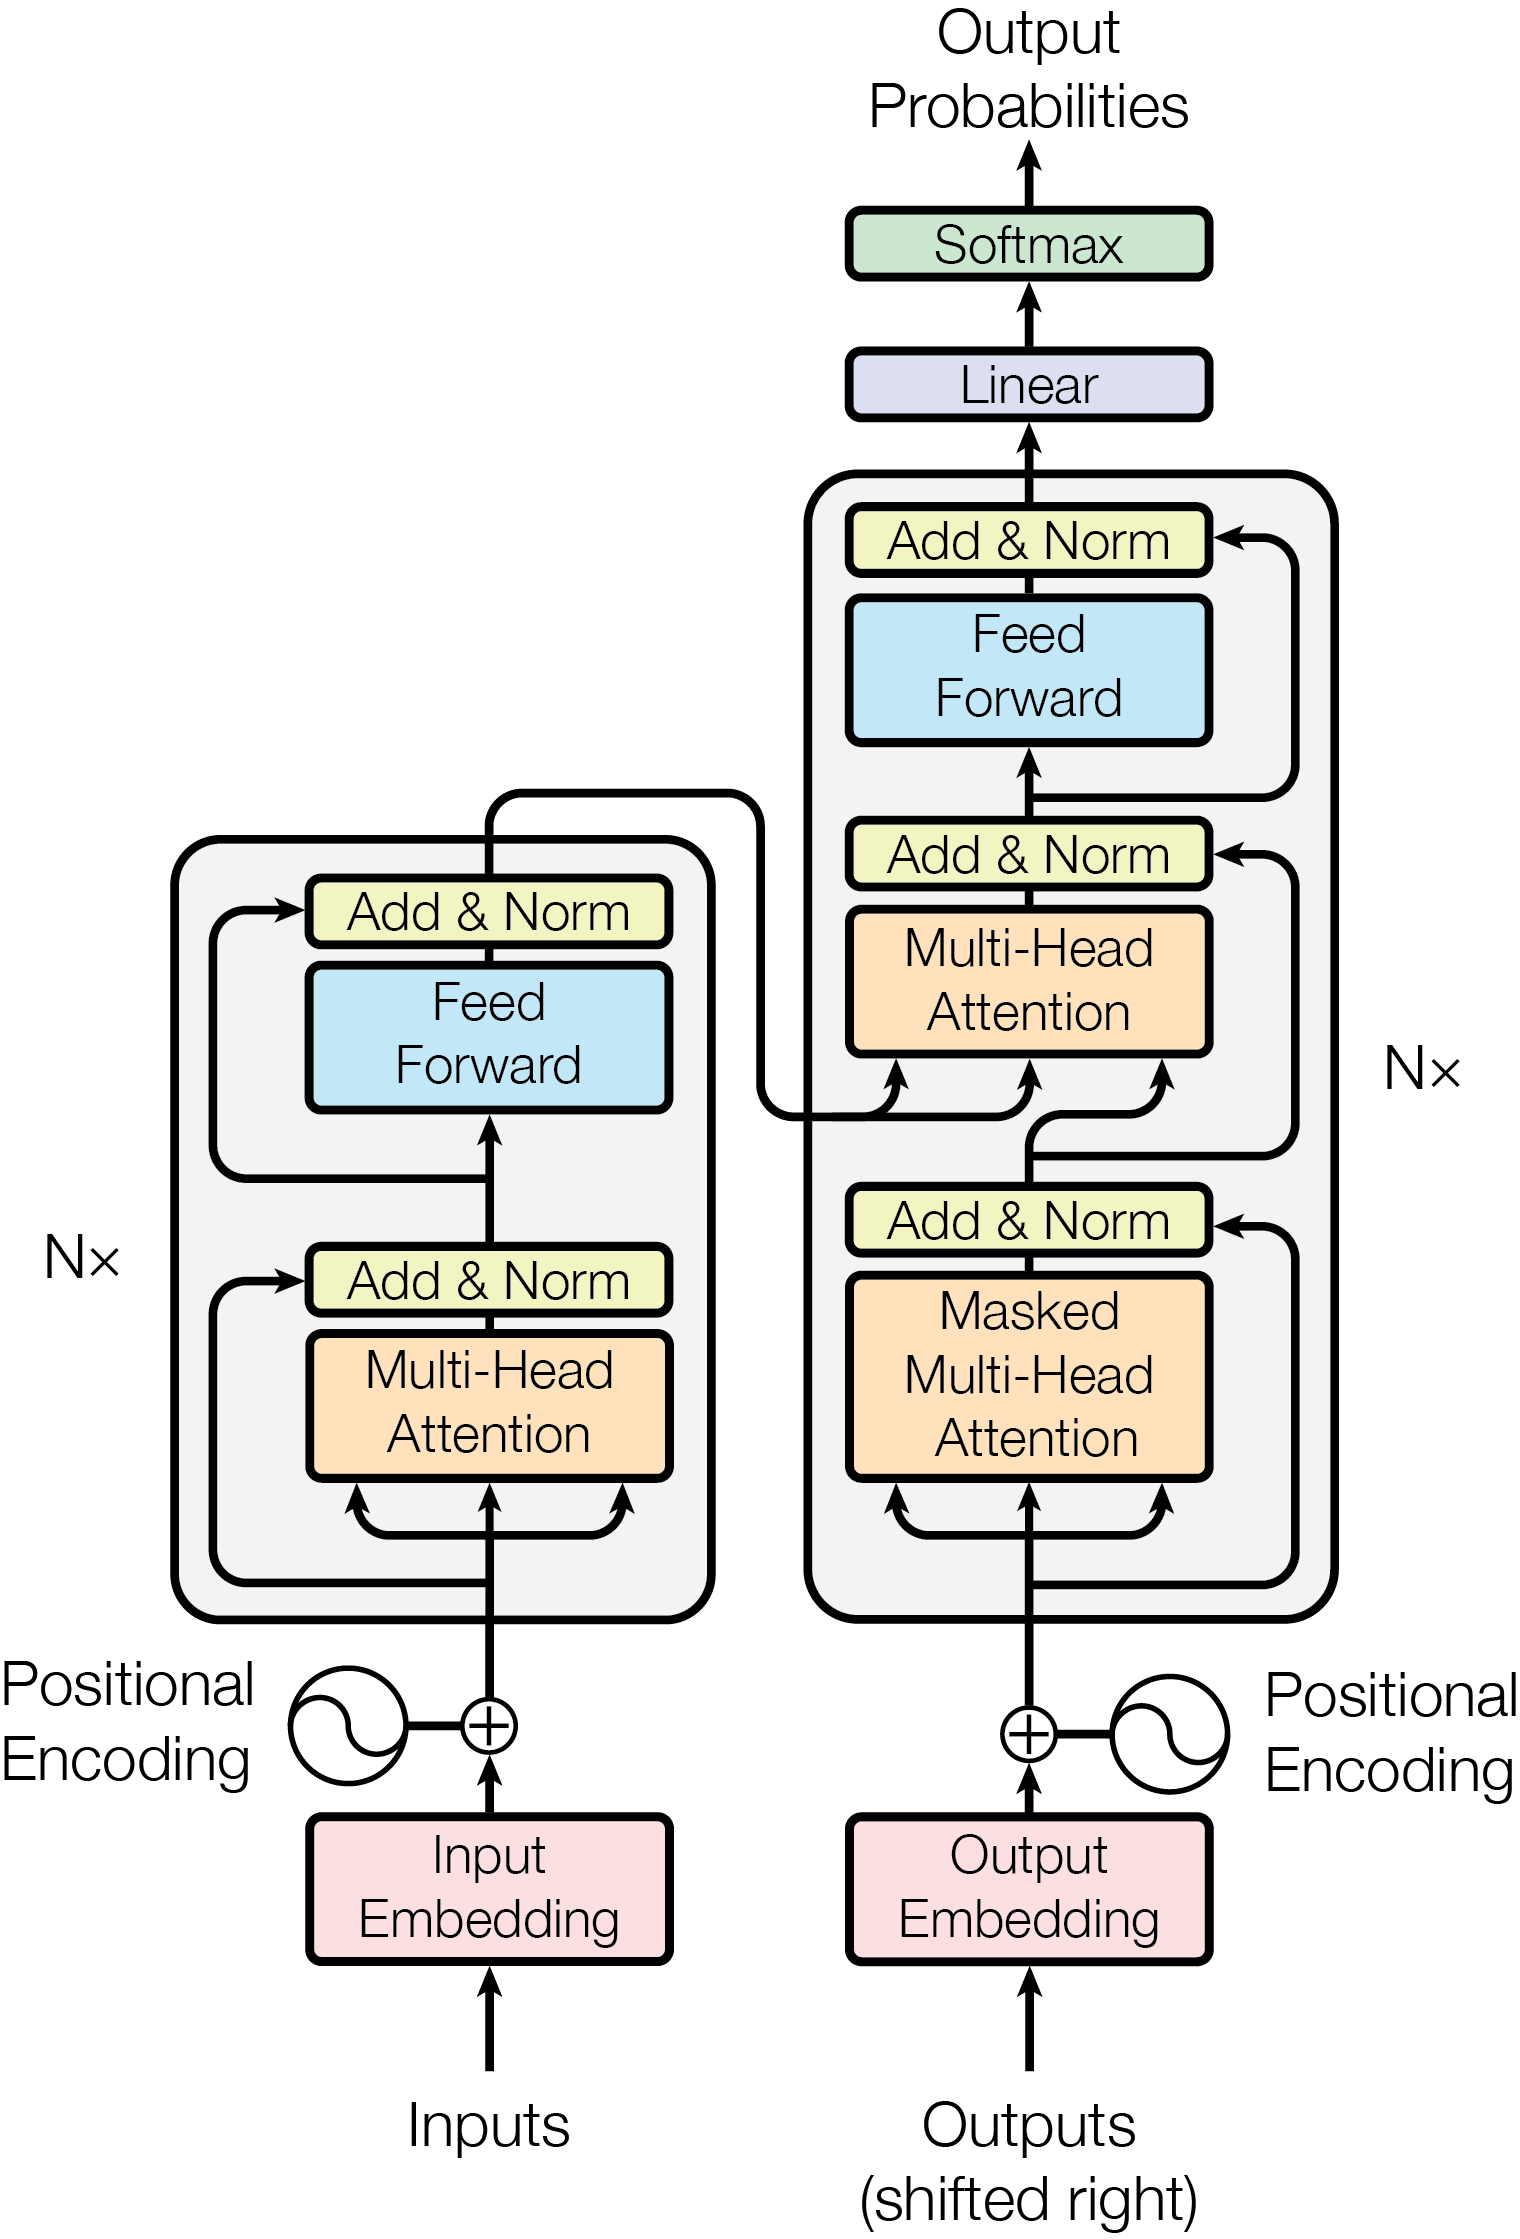
\includegraphics[width=6cm]{Graphics/transformer.png}
    \caption{Transformer model representation\cite{Vaswani_2017}.}
    \label{fig:transformer}
\end{figure}

\subsection{BERT}

BERT model is an acronym for Bidirectional Encoder Representations for Transformers. BERT alleviates the previously mentioned unidi rectionality constraint by using a `masked lan guage model' (MLM) pretraining objective, in spired by the Cloze task\cite{Taylor_1953}. The masked language model randomly masks some of the tokens from the input, and the objective is to predict the original vocabulary id of the masked word based only on its context. Pre-trained word embeddings are an integral part of modern NLP systems, offering significant improvements over embeddings learned from scratch\cite{Turian_2010}. To pre-train word embedding vectors, left-to-right language modeling objectives have been used\cite{Mnih_2008}, as well as objectives to discriminate correct from incorrect words in left and right context\cite{Mikolov_2014}. As with the feature-based approaches, the first works in this direction only pre-trained word embedding parameters from unlabeled text\cite{Collobert_2008}. More recently, sentence or document encoders which produce contextual token representations have been pre-trained from unlabeled text and fine-tuned for a supervised downstream task. The advantage of these approaches is that few parameters need to be learned from scratch.

\begin{figure}[H]
    \centering
    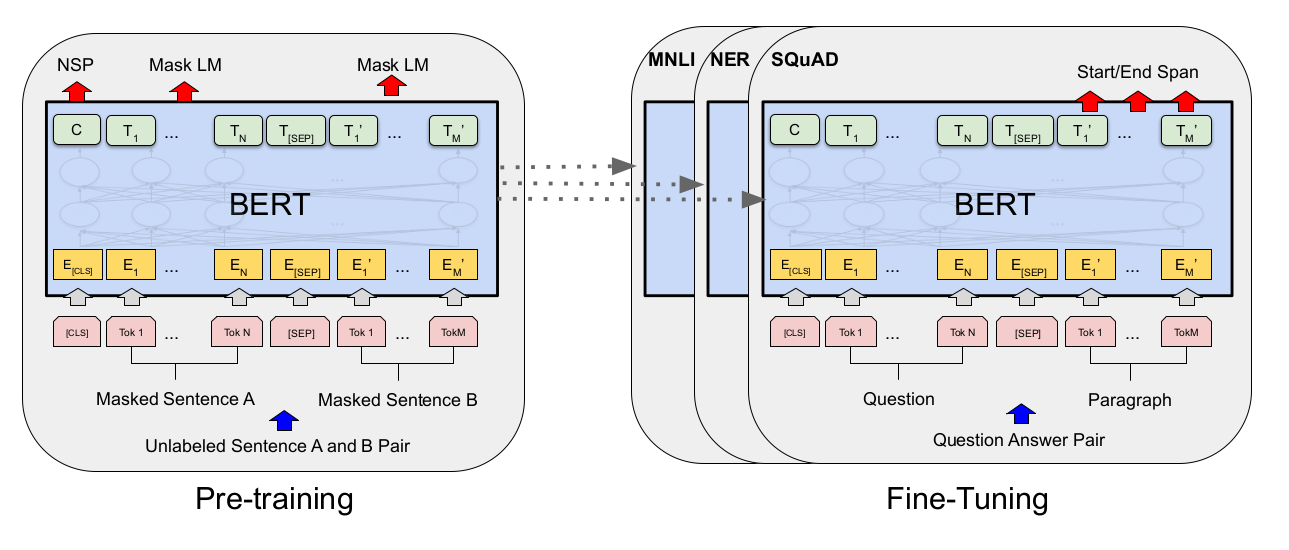
\includegraphics[width=13cm]{Graphics/bert.png}
    \caption{Overall pretraining and fine-tuning procedures for BERT. Apart from output layers, the same architectures are used in both pretraining and fine-tuning. The same pre-trained model parameters are used to initialize models for different down-stream tasks.\cite{Devlin_2018}}
    \label{fig:bert}
\end{figure}

There are two steps in our framework: pretraining and fine-tuning. During pretraining, the model is trained on unlabeled data over different pretraining tasks. For fine-tuning, the BERT model is first initialized with the pre-trained parameters, and all of the parameters are fine-tuned using labeled data from the downstream tasks. Each downstream task has separate fine-tuned models, even though they are initialized with the same pre-trained parameters. The question-answering example in Figure \ref{fig:bert} will serve as a running example for this section. To make BERT handle a variety of down-stream tasks, our input representation is able to unambiguously represent both a single sentence and a pair of sentences in one token sequence. Throughout this work, a sentence can be an arbitrary span of contiguous text, rather than an actual linguistic sentence.

\subsection{RoBERTa}

The BERT model can be optimized with some modifications on the pretraining procedure. Liu\cite{Liu_2019} join this configurations in one model named Robustly optimized BERT approach (RoBERTa). Especifically, RoBERTa is trained with dynamic masking, FULL-SENTENCES without NS loss, large mini-batches. One of the most important modifications is the number of training passes and the size of the bacth. This is because Large batch training can improve training efficiency even without large scale parallel hardware through gradient accumulation, whereby gradients from multiple mini-batches are accumulated locally before each optimization step\cite{Ott_2019}. In all the test that Liu\cite{Liu_2019} did in his paper demostrate that RoBERTa have a perfomance by training the model with bigger batches over more data, removing the next sentence prediction, training on longer sequences and dynamically changing the masking pattern applied to the traning data.

\subsection{RoBERTuito}

The RoBERTuito model has a RoBERTa base architecture. This model have 2 self-attention layers, 12 attention heads, and hidden size equal to 768, in the same fashion as BERTweet\cite{Nguyen_2020}. RoBERTuito use a masked language objective disregarding the next-sentence prediction task used in BERT or other tweet-order tasks such as those used in Gonzalez et al.\cite{Gonzalez_2021}.

\subsection{MEX-A3T}

\begin{table}[H]
    \centering
    \changefontsizes{9pt}
    \begin{tabular}{lrrrrrr} \hline
        \\
        \textbf{Team Name}          & \textbf{F1 offensive} & \textbf{F1 non-offensive} & \textbf{F1 macro} & \textbf{Precision} & \textbf{Recall} & \textbf{Accuracy} \\ \hline
        \\[-0.1cm]
        \textbf{CIMAT-1}            & 0.7998                & 0.9195                    & 0.8596            & 0.8605             & 0.8588          & 0.8851            \\[0.05cm]
        \textbf{CIMAT-2}            & 0.7971                & 0.9205                    & 0.8588            & 0.8641             & 0.8540          & 0.8858            \\[0.05cm]
        \textbf{UPB-2}              & 0.7969                & 0.9107                    & 0.8538            & 0.8440             & 0.8668          & 0.8759            \\[0.05cm]
        \textbf{UACh-2}             & 0.7720                & 0.9042                    & 0.8381            & 0.8332             & 0.8437          & 0.8651            \\[0.05cm]
        \textbf{INGEOTEC}           & 0.7468                & 0.8933                    & 0.8200            & 0.8150             & 0.8258          & 0.8498            \\[0.05cm]
        \textbf{Idiap-UAM-1}        & 0.7255                & 0.8886                    & 0.8071            & 0.8067             & 0.8075          & 0.8416            \\[0.05cm]
        \textbf{Baseline (Bi-GRU)}  & 0.7124                & 0.8841                    & 0.7983            & 0.7988             & 0.7978          & 0.8348            \\[0.05cm]
        \textbf{Idiap-UAM-2}        & 0.7066                & 0.8953                    & 0.8010            & 0.8234             & 0.7860          & 0.8457            \\[0.05cm]
        \textbf{UACh-1}             & 0.7062                & 0.8861                    & 0.7961            & 0.8021             & 0.7909          & 0.8358            \\[0.05cm]
        \textbf{DeepMath-1}         & 0.7001                & 0.8544                    & 0.7773            & 0.7662             & 0.8120          & 0.8040            \\[0.05cm]
        \textbf{DeepMath-2}         & 0.6957                & 0.8537                    & 0.7747            & 0.7639             & 0.7971          & 0.8024            \\[0.05cm]
        \textbf{Baseline (BoW-SVM)} & 0.6760                & 0.8780                    & 0.7770            & -                  & -               & 0.8228            \\[0.05cm]
        \textbf{UMUTeam-2}          & 0.6727                & 0.8706                    & 0.7716            & 0.7744             & 0.7691          & 0.8145            \\[0.05cm]
        \textbf{Intensos-1}         & 0.6619                & 0.8752                    & 0.7686            & 0.7820             & 0.7588          & 0.8177            \\[0.05cm]
        \textbf{UMUTeam-3}          & 0.6516                & 0.8771                    & 0.7644            & 0.7868             & 0.7503          & 0.8183            \\[0.05cm]
        \textbf{Ugalileo-2}         & 0.6388                & 0.8208                    & 0.7298            & 0.7213             & 0.7531          & 0.7604            \\[0.05cm]
        \textbf{Ugalileo-1}         & 0.6387                & 0.8430                    & 0.7408            & 0.7350             & 0.7486          & 0.7811            \\[0.05cm]
        \textbf{ITCG-SD}            & 0.6080                & 0.8820                    & 0.7450            & 0.8133             & 0.7203          & 0.8186            \\[0.05cm]
        \textbf{UMUTeam-1}          & 0.5892                & 0.8430                    & 0.7161            & 0.7223             & 0.7112          & 0.7728            \\[0.05cm]
        \textbf{UPB-1}              & 0.3437                & 0.8463                    & 0.5950            & 0.7333             & 0.5947          & 0.7509            \\[0.05cm]
        \textbf{Intensos-2}         & 0.2515                & 0.7664                    & 0.5090            & 0.5189             & 0.5141          & 0.6440            \\[0.05cm] \hline
    \end{tabular}
    \normalsize
    \caption{Results for aggressiveness identification in the IberLEF 2020.}
    \label{table:agIberLEF_2020}
\end{table}